% Options for packages loaded elsewhere
\PassOptionsToPackage{unicode}{hyperref}
\PassOptionsToPackage{hyphens}{url}
\PassOptionsToPackage{dvipsnames,svgnames,x11names}{xcolor}
%
\documentclass[
  letterpaper,
  DIV=11,
  numbers=noendperiod]{scrreprt}

\usepackage{amsmath,amssymb}
\usepackage{iftex}
\ifPDFTeX
  \usepackage[T1]{fontenc}
  \usepackage[utf8]{inputenc}
  \usepackage{textcomp} % provide euro and other symbols
\else % if luatex or xetex
  \usepackage{unicode-math}
  \defaultfontfeatures{Scale=MatchLowercase}
  \defaultfontfeatures[\rmfamily]{Ligatures=TeX,Scale=1}
\fi
\usepackage{lmodern}
\ifPDFTeX\else  
    % xetex/luatex font selection
\fi
% Use upquote if available, for straight quotes in verbatim environments
\IfFileExists{upquote.sty}{\usepackage{upquote}}{}
\IfFileExists{microtype.sty}{% use microtype if available
  \usepackage[]{microtype}
  \UseMicrotypeSet[protrusion]{basicmath} % disable protrusion for tt fonts
}{}
\makeatletter
\@ifundefined{KOMAClassName}{% if non-KOMA class
  \IfFileExists{parskip.sty}{%
    \usepackage{parskip}
  }{% else
    \setlength{\parindent}{0pt}
    \setlength{\parskip}{6pt plus 2pt minus 1pt}}
}{% if KOMA class
  \KOMAoptions{parskip=half}}
\makeatother
\usepackage{xcolor}
\setlength{\emergencystretch}{3em} % prevent overfull lines
\setcounter{secnumdepth}{5}
% Make \paragraph and \subparagraph free-standing
\makeatletter
\ifx\paragraph\undefined\else
  \let\oldparagraph\paragraph
  \renewcommand{\paragraph}{
    \@ifstar
      \xxxParagraphStar
      \xxxParagraphNoStar
  }
  \newcommand{\xxxParagraphStar}[1]{\oldparagraph*{#1}\mbox{}}
  \newcommand{\xxxParagraphNoStar}[1]{\oldparagraph{#1}\mbox{}}
\fi
\ifx\subparagraph\undefined\else
  \let\oldsubparagraph\subparagraph
  \renewcommand{\subparagraph}{
    \@ifstar
      \xxxSubParagraphStar
      \xxxSubParagraphNoStar
  }
  \newcommand{\xxxSubParagraphStar}[1]{\oldsubparagraph*{#1}\mbox{}}
  \newcommand{\xxxSubParagraphNoStar}[1]{\oldsubparagraph{#1}\mbox{}}
\fi
\makeatother

\usepackage{color}
\usepackage{fancyvrb}
\newcommand{\VerbBar}{|}
\newcommand{\VERB}{\Verb[commandchars=\\\{\}]}
\DefineVerbatimEnvironment{Highlighting}{Verbatim}{commandchars=\\\{\}}
% Add ',fontsize=\small' for more characters per line
\usepackage{framed}
\definecolor{shadecolor}{RGB}{241,243,245}
\newenvironment{Shaded}{\begin{snugshade}}{\end{snugshade}}
\newcommand{\AlertTok}[1]{\textcolor[rgb]{0.68,0.00,0.00}{#1}}
\newcommand{\AnnotationTok}[1]{\textcolor[rgb]{0.37,0.37,0.37}{#1}}
\newcommand{\AttributeTok}[1]{\textcolor[rgb]{0.40,0.45,0.13}{#1}}
\newcommand{\BaseNTok}[1]{\textcolor[rgb]{0.68,0.00,0.00}{#1}}
\newcommand{\BuiltInTok}[1]{\textcolor[rgb]{0.00,0.23,0.31}{#1}}
\newcommand{\CharTok}[1]{\textcolor[rgb]{0.13,0.47,0.30}{#1}}
\newcommand{\CommentTok}[1]{\textcolor[rgb]{0.37,0.37,0.37}{#1}}
\newcommand{\CommentVarTok}[1]{\textcolor[rgb]{0.37,0.37,0.37}{\textit{#1}}}
\newcommand{\ConstantTok}[1]{\textcolor[rgb]{0.56,0.35,0.01}{#1}}
\newcommand{\ControlFlowTok}[1]{\textcolor[rgb]{0.00,0.23,0.31}{\textbf{#1}}}
\newcommand{\DataTypeTok}[1]{\textcolor[rgb]{0.68,0.00,0.00}{#1}}
\newcommand{\DecValTok}[1]{\textcolor[rgb]{0.68,0.00,0.00}{#1}}
\newcommand{\DocumentationTok}[1]{\textcolor[rgb]{0.37,0.37,0.37}{\textit{#1}}}
\newcommand{\ErrorTok}[1]{\textcolor[rgb]{0.68,0.00,0.00}{#1}}
\newcommand{\ExtensionTok}[1]{\textcolor[rgb]{0.00,0.23,0.31}{#1}}
\newcommand{\FloatTok}[1]{\textcolor[rgb]{0.68,0.00,0.00}{#1}}
\newcommand{\FunctionTok}[1]{\textcolor[rgb]{0.28,0.35,0.67}{#1}}
\newcommand{\ImportTok}[1]{\textcolor[rgb]{0.00,0.46,0.62}{#1}}
\newcommand{\InformationTok}[1]{\textcolor[rgb]{0.37,0.37,0.37}{#1}}
\newcommand{\KeywordTok}[1]{\textcolor[rgb]{0.00,0.23,0.31}{\textbf{#1}}}
\newcommand{\NormalTok}[1]{\textcolor[rgb]{0.00,0.23,0.31}{#1}}
\newcommand{\OperatorTok}[1]{\textcolor[rgb]{0.37,0.37,0.37}{#1}}
\newcommand{\OtherTok}[1]{\textcolor[rgb]{0.00,0.23,0.31}{#1}}
\newcommand{\PreprocessorTok}[1]{\textcolor[rgb]{0.68,0.00,0.00}{#1}}
\newcommand{\RegionMarkerTok}[1]{\textcolor[rgb]{0.00,0.23,0.31}{#1}}
\newcommand{\SpecialCharTok}[1]{\textcolor[rgb]{0.37,0.37,0.37}{#1}}
\newcommand{\SpecialStringTok}[1]{\textcolor[rgb]{0.13,0.47,0.30}{#1}}
\newcommand{\StringTok}[1]{\textcolor[rgb]{0.13,0.47,0.30}{#1}}
\newcommand{\VariableTok}[1]{\textcolor[rgb]{0.07,0.07,0.07}{#1}}
\newcommand{\VerbatimStringTok}[1]{\textcolor[rgb]{0.13,0.47,0.30}{#1}}
\newcommand{\WarningTok}[1]{\textcolor[rgb]{0.37,0.37,0.37}{\textit{#1}}}

\providecommand{\tightlist}{%
  \setlength{\itemsep}{0pt}\setlength{\parskip}{0pt}}\usepackage{longtable,booktabs,array}
\usepackage{calc} % for calculating minipage widths
% Correct order of tables after \paragraph or \subparagraph
\usepackage{etoolbox}
\makeatletter
\patchcmd\longtable{\par}{\if@noskipsec\mbox{}\fi\par}{}{}
\makeatother
% Allow footnotes in longtable head/foot
\IfFileExists{footnotehyper.sty}{\usepackage{footnotehyper}}{\usepackage{footnote}}
\makesavenoteenv{longtable}
\usepackage{graphicx}
\makeatletter
\def\maxwidth{\ifdim\Gin@nat@width>\linewidth\linewidth\else\Gin@nat@width\fi}
\def\maxheight{\ifdim\Gin@nat@height>\textheight\textheight\else\Gin@nat@height\fi}
\makeatother
% Scale images if necessary, so that they will not overflow the page
% margins by default, and it is still possible to overwrite the defaults
% using explicit options in \includegraphics[width, height, ...]{}
\setkeys{Gin}{width=\maxwidth,height=\maxheight,keepaspectratio}
% Set default figure placement to htbp
\makeatletter
\def\fps@figure{htbp}
\makeatother
% definitions for citeproc citations
\NewDocumentCommand\citeproctext{}{}
\NewDocumentCommand\citeproc{mm}{%
  \begingroup\def\citeproctext{#2}\cite{#1}\endgroup}
\makeatletter
 % allow citations to break across lines
 \let\@cite@ofmt\@firstofone
 % avoid brackets around text for \cite:
 \def\@biblabel#1{}
 \def\@cite#1#2{{#1\if@tempswa , #2\fi}}
\makeatother
\newlength{\cslhangindent}
\setlength{\cslhangindent}{1.5em}
\newlength{\csllabelwidth}
\setlength{\csllabelwidth}{3em}
\newenvironment{CSLReferences}[2] % #1 hanging-indent, #2 entry-spacing
 {\begin{list}{}{%
  \setlength{\itemindent}{0pt}
  \setlength{\leftmargin}{0pt}
  \setlength{\parsep}{0pt}
  % turn on hanging indent if param 1 is 1
  \ifodd #1
   \setlength{\leftmargin}{\cslhangindent}
   \setlength{\itemindent}{-1\cslhangindent}
  \fi
  % set entry spacing
  \setlength{\itemsep}{#2\baselineskip}}}
 {\end{list}}
\usepackage{calc}
\newcommand{\CSLBlock}[1]{\hfill\break\parbox[t]{\linewidth}{\strut\ignorespaces#1\strut}}
\newcommand{\CSLLeftMargin}[1]{\parbox[t]{\csllabelwidth}{\strut#1\strut}}
\newcommand{\CSLRightInline}[1]{\parbox[t]{\linewidth - \csllabelwidth}{\strut#1\strut}}
\newcommand{\CSLIndent}[1]{\hspace{\cslhangindent}#1}

\KOMAoption{captions}{tableheading}
\makeatletter
\@ifpackageloaded{tcolorbox}{}{\usepackage[skins,breakable]{tcolorbox}}
\@ifpackageloaded{fontawesome5}{}{\usepackage{fontawesome5}}
\definecolor{quarto-callout-color}{HTML}{909090}
\definecolor{quarto-callout-note-color}{HTML}{0758E5}
\definecolor{quarto-callout-important-color}{HTML}{CC1914}
\definecolor{quarto-callout-warning-color}{HTML}{EB9113}
\definecolor{quarto-callout-tip-color}{HTML}{00A047}
\definecolor{quarto-callout-caution-color}{HTML}{FC5300}
\definecolor{quarto-callout-color-frame}{HTML}{acacac}
\definecolor{quarto-callout-note-color-frame}{HTML}{4582ec}
\definecolor{quarto-callout-important-color-frame}{HTML}{d9534f}
\definecolor{quarto-callout-warning-color-frame}{HTML}{f0ad4e}
\definecolor{quarto-callout-tip-color-frame}{HTML}{02b875}
\definecolor{quarto-callout-caution-color-frame}{HTML}{fd7e14}
\makeatother
\makeatletter
\@ifpackageloaded{bookmark}{}{\usepackage{bookmark}}
\makeatother
\makeatletter
\@ifpackageloaded{caption}{}{\usepackage{caption}}
\AtBeginDocument{%
\ifdefined\contentsname
  \renewcommand*\contentsname{Table of contents}
\else
  \newcommand\contentsname{Table of contents}
\fi
\ifdefined\listfigurename
  \renewcommand*\listfigurename{List of Figures}
\else
  \newcommand\listfigurename{List of Figures}
\fi
\ifdefined\listtablename
  \renewcommand*\listtablename{List of Tables}
\else
  \newcommand\listtablename{List of Tables}
\fi
\ifdefined\figurename
  \renewcommand*\figurename{Figure}
\else
  \newcommand\figurename{Figure}
\fi
\ifdefined\tablename
  \renewcommand*\tablename{Table}
\else
  \newcommand\tablename{Table}
\fi
}
\@ifpackageloaded{float}{}{\usepackage{float}}
\floatstyle{ruled}
\@ifundefined{c@chapter}{\newfloat{codelisting}{h}{lop}}{\newfloat{codelisting}{h}{lop}[chapter]}
\floatname{codelisting}{Listing}
\newcommand*\listoflistings{\listof{codelisting}{List of Listings}}
\makeatother
\makeatletter
\makeatother
\makeatletter
\@ifpackageloaded{caption}{}{\usepackage{caption}}
\@ifpackageloaded{subcaption}{}{\usepackage{subcaption}}
\makeatother

\ifLuaTeX
  \usepackage{selnolig}  % disable illegal ligatures
\fi
\usepackage{bookmark}

\IfFileExists{xurl.sty}{\usepackage{xurl}}{} % add URL line breaks if available
\urlstyle{same} % disable monospaced font for URLs
\hypersetup{
  pdftitle={Basics of sustainability},
  pdfauthor={Christoph Bader},
  colorlinks=true,
  linkcolor={blue},
  filecolor={Maroon},
  citecolor={Blue},
  urlcolor={Blue},
  pdfcreator={LaTeX via pandoc}}


\title{Basics of sustainability}
\usepackage{etoolbox}
\makeatletter
\providecommand{\subtitle}[1]{% add subtitle to \maketitle
  \apptocmd{\@title}{\par {\large #1 \par}}{}{}
}
\makeatother
\subtitle{Foundations and Challenges of sustainability}
\author{Christoph Bader}
\date{Invalid Date}

\begin{document}
\maketitle

\renewcommand*\contentsname{Table of contents}
{
\hypersetup{linkcolor=}
\setcounter{tocdepth}{2}
\tableofcontents
}

\bookmarksetup{startatroot}

\chapter*{Preface}\label{preface}
\addcontentsline{toc}{chapter}{Preface}

\markboth{Preface}{Preface}

This is a Quarto book.

To learn more about Quarto books visit
\url{https://quarto.org/docs/books}.

\begin{Shaded}
\begin{Highlighting}[]
\DecValTok{1} \SpecialCharTok{+} \DecValTok{1}
\end{Highlighting}
\end{Shaded}

\begin{verbatim}
[1] 2
\end{verbatim}

\bookmarksetup{startatroot}

\chapter{Introduction}\label{introduction}

Amid the mounting challenges of sustainable development, Christo and
Jeanne-Claude's ``Wrapped Globe'' is a powerful symbol of humanity's
responsibility towards our planet and its resources. The artwork depicts
a globe wrapped in transparent plastic and a filigree net. Meanwhile, in
real life, the world is facing a ``polycrisis'' -- the word used to
describe the many serious crises our Earth is facing, including
ecological crises, growing inequality, excessive national debt, and the
effects of the Covid-19 pandemic, to name but a few. In a polycrisis,
crises are increasingly intertwined and mutually reinforcing (Tooze
2022), and they are mainly caused by a structural dependence on growth
(as measured by gross domestic product, GDP) (Hickel et al., 2022;
Sennholz, 2021); a vicious circle of ever-increasing concentration of
economic and political power in the hands of a few (Piketty, 2014); and
persistent inequalities between and within countries (Chancel et al.,
2021; Milanovic, 2016). And yet, we keep striving for GDP growth in our
society and our economy, in order to maintain and create jobs, finance
our social security systems, secure tax revenues, and fulfil the needs
of companies and industries that depend on growth to exist. As these
expectations become increasingly unrealistic, the idea of decoupling
economic growth from resource consumption has gained traction. However,
there is no empirical evidence that doing so will achieve anywhere near
the scale required to halt multidimensional ecological collapse
(Parrique et al., 2019; Hickel and Kallis, 2020; Wiedmann et al., 2020).

\section{Full and empty world}\label{full-and-empty-world}

The plastic cover and the net wrapped around Christo's globe thus
represent the interconnectedness and interdependence of the Earth's
various elements, and emphasize the need to maintain and preserve these
relationships. A similar idea was described by the economist Herman Daly
(2015), who put forth a concept of the ``empty'' and the ``full'' world.
The empty world describes a situation in which human activities and
resource use have only a minor impact on the environment. In this world,
natural systems are still intact and untouched, and resources are
sufficient to meet human needs. This contrasts with the full world, in
which human activities and resource use overload the ecosystem and
pollute the environment. Since at least the Second World War, we have
pursued an industrialized society and a growth economy. As a result, we
now live in a ``full'' world, where natural resources are scarce and the
balance of ecosystems is under threat. Daly's epiphany came in 1962 upon
reading Rachel Carson's book, Silent Spring, which called for a life in
harmony with nature. Daly was already sceptical about the
hyper-individualism of economic models, and Carson's work highlighted
the conflict between a growing economy and a fragile environment.
Following a lecture by the economist Nicholas Georgescu-Roegen on his
magnum opus, The Entropy Law and the Economic Process (1971), Daly
adopted the idea that the economy was more like an hourglass than a
pendulum, with valuable resources turning into waste and thus largely
irreversibly lost. There is no master plan to counter the polycrisis and
make our economic and social system more sustainable.

\section{This book}\label{this-book}

To contribute to sustainable development, we need to analyse the causes
of symptoms such as biodiversity loss or global warming, and learn to
understand how they are connected and how they interact. We will
therefore look at current problems and challenges such as global
warming, pollution, biodiversity loss, social inequality, and economic
disparities, to understand how they can be tackled at both the local and
the global level. The aim of this textbook is to encourage readers to
think critically about the role of individuals, communities, businesses,
and governments in the context of sustainable development -- and thus to
identify and pursue approaches to support sustainable development. In
addition, we want to develop visions of the future, especially in the
Master's study programmes, that make it possible to imagine a high
quality of life in a sustainable modern age, and that make changing the
present seem attractive rather than daunting. We want to envision a
different food culture, a different economic system, a different type of
land use, and a different way of building and living. To make progress
towards sustainability, it will be critical to engage stakeholders and
foster collaboration across sectors and disciplines. As this textbook
will emphasize, education, communication, and participation will also be
indispensable in shaping a more sustainable future. With Christo's
Wrapped Globe in mind, and Daly's understanding of the empty and the
full world as a foundation, we will embark on a journey through the many
aspects of sustainable development. We hope that you will find this
journey both informative and inspiring, and that it will give you an
understanding of both the urgency and the opportunities for sustainable
development.

Finally, we hope that our study programmes will inspire students to
reflect on their own roles and responsibilities in relation to
sustainability, and that it will equip you to make a difference to
ensure that the Earth remains a place worth living in for future
generations. Only together can we bring about the changes needed to
create a sustainable, just, and environmentally friendly world.

\part{Understanding and concepts}

\part{Understandings and concepts of sustainability}

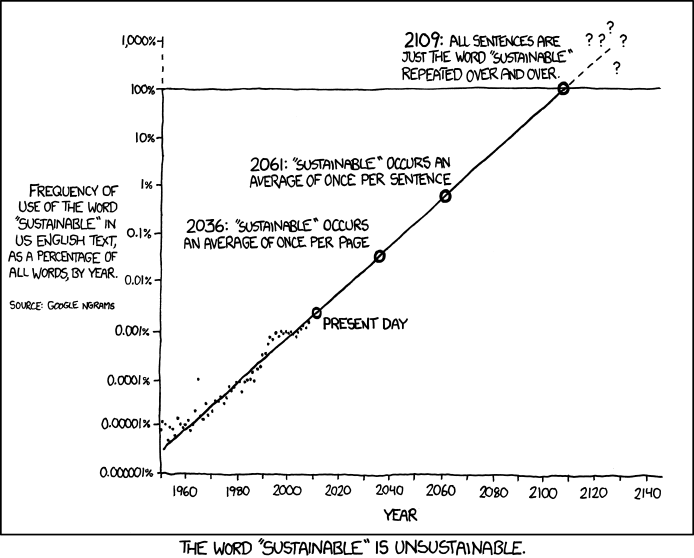
\includegraphics{1_understanding/images/sustainable-01.png}Is the term
``Sustainability'' so overused as to slowly become meaningless? Even if
this is the case, we shouldn't abandon key terms like this lightly. For
example, it's still important for companies to have a sustainability
strategy, even if many such strategies are inadequate or amount to
greenwashing. We need to clarify the meaning of ``sustainability'' and
hold those who use it to account. And we should base our interpretation
on science and historical developments. The historical precursors to the
sustainability model explained in this textbook are:

\begin{itemize}
\item
  Start of the discussion about sustainability: Carlowitz's forest
  management principle of 1713
\item
  Clash of economy and ecology First and second UN Development Decades
  (1960s and 1970s)
\item
  The Limits to Growth (1972)
\item
  Brundtland Report (1987)
\item
  Rio Earth Summit 1992 Agenda 21 UN Millennium Development Goals (MDGs)
  (2000--2015)
\item
  2030 Agenda with the Sustainable Development Goals (SDGs) (2015--2030)
\end{itemize}

\chapter{Sustainability?}\label{sustainability}

Where do the concept, mission statement, and guiding principles of
sustainable development come from? How did the concept emerge, how did
it evolve -- and why? The following explanations provide an overview of
the history of sustainability, the political background, and key
conferences and documents. In short, what has made sustainability what
it is today. It's about seeing the big picture. Because only those who
know the past can assess the future. Sustainability has been the
buzzword of recent years, from science to politics and business to the
media. Initially, the term has a positive connotation because it is
associated with the long term, the durable, and many things are
sustainable today: coffee, corporate philosophy, even tuna pizzas. These
are the demands of a consumer society with an inconsiderate appetite for
abundance. First thing in the morning, the shampoo removes our dandruff
``sustainably''. Then we drive to work at a company that prides itself
on its ``sustainable corporate philosophy'', and over lunch we discuss
sustainable investments. At home, we stick a tuna pizza in the oven --
sustainably sourced and produced, of course, as it says on the box.
Today, the term ``sustainability'' is everywhere: it's used in
connection with energy, mobility, building renovation, nutrition,
population development, corporate environmental management, and climate
protection. It's also used in art, culture, design, and advertising.

\chapter{A normative concept}\label{a-normative-concept}

To achieve sustainability, we need sustainable development: a strategic
process that requires changes in our socio-ecological systems and
institutions. ``Development'' implies controlled improvement, and the
ethical question of what exactly ``better'' means is key. The use of the
term ``development'' has been criticized by some (e.g.~Lang et al.~2014;
Kothari et al.~2019), as it is often equated with unbridled growth.
Unbridled growth of the ``ecological footprint'' -- the proportion of
the biosphere used for human production, consumption, and waste -- is
unsustainable in the long term. Nonetheless, there are different
interpretations of ``development'', ranging from economic growth to
improving quality of life. Sustainable development therefore remains a
stimulating and controversial concept. Sustainability and sustainable
development play a key role in today's political discourse. The term
``unsustainability'' refers to conditions or developments that are
considered negative, while ``sustainability'' represents a positive
state.

The concept of sustainable development commits us to certain values and
norms that define ethical goals and rules of behaviour. These values and
norms shape our ideas of what we consider a desirable or ``positive''
change. A neutral point of view is not possible, as our perceptions are
shaped by a variety of influences. Our personal experiences, upbringing,
social environment, and cultural background all influence how we see and
interpret the world, including our perceptions of what ``should be'' and
what actions ``should be taken''. Ethics play a key role in determining
how the current situation can be improved to achieve sustainability, by
defining normative goals and limits. Sustainable development is
therefore a conceptual framework that is strongly driven by ethical
considerations.

Sustainability challenges such as poverty reduction and climate change
are therefore ethical challenges. The identification of situations as
sustainability problems (and therefore as ``negative'') and the choice
of solutions are based on ethical values. Sustainability goals are also
based on ethical values, as well as on knowledge of cause-and-effect
relationships. Sustainability issues are often referred to as ``wicked
problems'', because of their complex and pluralistic nature. Global
warming, in particular, has been described as a ``super wicked
problem'', as finding solutions is urgent, political institutions are
often inadequate, and decision-making processes suffer from
short-sightedness.

\section{Global challenges as wicked
problems}\label{global-challenges-as-wicked-problems}

Mike Hulme, author of Why We Disagree About Climate Change (2009),
suggests that we view climate change as a ``wicked problem'' of enormous
scale and likely longevity. This approach helps us see climate change
not as a problem that needs to be solved, but as a condition in which we
are directly involved. The categorization of problems as ``wicked'',
i.e.~those that do not lend themselves to clear-cut solutions,
originated with the planning theorists Horst Rittl and Melvin Webber
(1973). They argued that planners have to deal with unpredictable human
behaviour, and that some problems are too complicated to be solved
completely. Some ``wicked problems'' may never be fully solved, but we
can learn to cope with them and not let them dominate us.

\begin{tcolorbox}[enhanced jigsaw, toprule=.15mm, breakable, opacityback=0, arc=.35mm, colback=white, rightrule=.15mm, bottomrule=.15mm, colframe=quarto-callout-note-color-frame, left=2mm, leftrule=.75mm]

\vspace{-3mm}\textbf{Wicked problems}\vspace{3mm}

According to Bannink and Trommel (2019), wicked problems arise at the
intersection of factual uncertainty and a heterogeneity of preferences
and interests. Wicked problems are characterized by (Rittel \& Weber,
1973; Alford, 2017; Sediri, 2020):

\begin{itemize}
\item
  Complexity: Wicked problems are characterized by many interrelated
  factors and interactions. There are no clear cause-and-effect
  relationships, and changes in one area can have unforeseen effects in
  other areas.
\item
  Normative conflicts: Wicked problems are perceived and interpreted
  differently by different stakeholders and interest groups. There is no
  clear definition or consensus on what exactly the problem is, or how
  it should be solved.
\item
  Interdisciplinarity: Wicked problems require an interdisciplinary
  approach as they involve different topics, perspectives, and
  stakeholders. Finding a solution often requires the cooperation and
  coordination of different disciplines and experts. Uncertainty:
  Incorrect, missing, or inaccessible information about the problem
  situation and about the continuity of the values of the variables
  involved.
\item
  No definitive solution: Wicked problems defy clear-cut solutions. They
  are dynamic, change over time, and require continuous adjustment and
  iterations. Examples of wicked problems include climate change,
  poverty alleviation, global health, and sustainability. The complexity
  and interaction of different factors in these areas make it difficult
  to find simple and clear-cut solutions. Dealing with wicked problems
  requires a high degree of reflection, collaboration, and the use of
  systemic thinking methods.
\end{itemize}

\end{tcolorbox}

How have we manoeuvred ourselves into the current situation, where
wicked problems pose such a challenge to sustainable development? In
this textbook, we will analyse and learn to understand three key global
challenges:

\begin{itemize}
\item
  the emergence of human-induced global warming;
\item
  the persistence of global poverty and rising inequalities;
\item
  and the threat of species extinction and overexploitation of natural
  resources.
\end{itemize}

The debate about human influence on global warming and climate change
has intensified since the publications of the Intergovernmental Panel on
Climate Change (IPCC). The driving force behind global warming is our
dependence on oil and other fossil fuels for transport, (electricity)
generation, agriculture, and many everyday products. Another wicked
problem is global poverty. Although there have been global efforts to
reduce poverty for decades, the globalized market economy often leads to
increased poverty in certain regions, and the gap between rich and poor
seems to be widening overall (Chancel et al., 2021). High-income
countries have maintained their prosperity and living standards at the
expense of others. These are ``externalized costs'', and they include
environmental degradation. For example, the wealth and living standards
of high-income countries are largely responsible for the threat of
species extinction and the overuse of natural resources (Lessenich,
2018). In addition to the abovementioned ``big three'' -- climate
change, poverty, and biodiversity loss -- there are many other global
sustainability challenges, such as deforestation, desertification,
declining soil fertility, dwindling fish stocks, pollution, wars,
conflicts, and increasing migration. In analysing these comprehensive
challenges we must also consider the temporal dimension. In 2004, graphs
depicting socio-economic and Earth system trends from 1750 to 2000 were
first published, revealing a dramatic upsurge and aptly termed ``The
Great Acceleration'' (Steffen et al., 2004).

The Great Acceleration described the exponential growth dynamics that
occurred after the Industrial Revolution, which led to a surge in
productivity in the mode of production and a significant increase in
material wealth. At the same time, but to a much lesser extent, there
was a massive increase in natural resource consumption and emissions.
Socio-economic growth went hand in hand with the acceleration of
biophysical trends. Figures 6 and 7 describe some examples of important
biophysical and socio-economic indicators, all of which start to
increase with the Industrial Revolution. From the middle of the 20th
century, the trend towards exponential growth becomes apparent.

\begin{tcolorbox}[enhanced jigsaw, toprule=.15mm, breakable, opacityback=0, arc=.35mm, colback=white, rightrule=.15mm, bottomrule=.15mm, colframe=quarto-callout-tip-color-frame, left=2mm, leftrule=.75mm]

\vspace{-3mm}\textbf{An illustration of exponential growth}\vspace{3mm}

The Wheat and Chessboard Problem is a mathematical problem often used to
illustrate the concept of exponential growth. In the story, a servant
asks the king to fill every square on a chessboard with grains of wheat,
doubling the number on each square. Growth starts slowly, but with each
doubling, the number of grains increases exponentially. By the 50th
square, the number of rice grains would be large enough to cover
Berlin's 365-metre-high television tower on Alexanderplatz. This story
illustrates the immense power of exponential growth and its impressive
results. Understanding the concept of exponential growth is crucial to
analysing phenomena such as population growth, technological progress,
environmental change, and the spread of disease. It illustrates how even
small changes or developments in a system can have a significant impact.
History reminds us that we need to think carefully about how we manage
such growth and the long-term consequences it can have.

\end{tcolorbox}

Resource extraction has increased significantly in recent decades, from
22 billion tonnes in 1970 to 70 billion tonnes in 2010 (UNEP, 2016).
Global warming is another pressing issue. The latest IPCC report (IPCC,
2023) predicts an increase in global average temperature of between 1.5
and 5.8 degrees Celsius, depending on the scenario and future emissions.
Another alarming phenomenon is deforestation. Every two seconds, an area
of forest the size of a football field is cut down -- an area the size
of New York City every day. And then there is the decline in
biodiversity, marked by the extinction of animal and plant species,
which threatens the ecological diversity of our planet. The Great
Acceleration (Figures 6 and 7) describes the observable and measurable
(negative) developments of key socio-economic and biophysical indicators
since 1950. The causes of these negative developments can be far removed
from the place where the problems arise or become most evident. For
example, job losses in one country may be caused by a multinational
company's decision to relocate part of its operations to another
country, in order to maximize profits. We cannot hope to fix such issues
unless we understand how the system -- in this case, the globalized
economy -- works. Similarly, we need to understand the Earth's global
climate systems to imagine what the consequences of global warming might
be in a particular area or region. This is why many of the methods and
concepts of sustainability science require systemic thinking. A systemic
thinking approach often begins with brainstorming to create a ``rich
picture'' of all the factors you need to consider in order to understand
the current behaviour of the system in question. For example, in the
case of a multinational company closing a particular business unit,
these would be the factors that might influence the decision to
continue, expand, or close certain business units. While an initial
mapping might look overly complex or even messy, creating a linear
flowchart can help clarify the flows of inputs and influences. This kind
of mapping may already reveal opportunities to reassess the relevant
influences and redesign the system to avoid unwanted outcomes. However,
further work may be required to develop ``conceptual models'' of the
system that identify unforeseen opportunities for improvement.
Incorporating systemic thinking into the methods and concepts of
sustainability science enables us to tackle the complexity of problems
and develop sound strategies for sustainable development. Systemic
thinking thus provides an important basis for understanding and shaping
the different understandings and concepts of sustainable development, as
the next chapter discusses in more detail.

\part{Approaches}

\chapter{planetary-boundaries}\label{planetary-boundaries}

\part{3\_ecological-sustainability/1\_intro.qmd}

\chapter{climate-system-and-ecosystems}\label{climate-system-and-ecosystems}

\part{Social Sustainability}

\chapter{normativity}\label{normativity}

\part{Economic Sustainability}

\chapter{normativity}\label{normativity-1}

\cleardoublepage
\phantomsection
\addcontentsline{toc}{part}{Appendices}
\appendix

\chapter*{References}\label{references}
\addcontentsline{toc}{chapter}{References}

\markboth{References}{References}

\phantomsection\label{refs}
\begin{CSLReferences}{1}{0}
\bibitem[\citeproctext]{ref-tooze2022}
Tooze, Adam. 2022. {``Welcome to the World of the Polycrisis.''}
\emph{Financial Times}, October.

\end{CSLReferences}




\end{document}
